\clearpage
\twocolumn[{%
\rqparent
\subsection{Scaling predictability}
\label{app:rq01_scaling_predictability}

\noindent\begin{minipage}[t]{0.485\textwidth}
\vspace{0pt}
\paragraph{Research Question.} \emph{Which benchmarks, and which per-language measurements, move with model size in a way a log-linear fit captures, so that a small-model measurement has a trend to extrapolate from at all?}

\paragraph{Setup.} We measure how predictably a task's score changes with model size and along training: the R$^2$ and the Spearman $\rho$ of log-linear fits. We use the deep cells with the baseline data (scheme A, T = 1) at seed 1904, 90M--1.7B, at every language setting. The tasks are every benchmark task in a trained language, gated above chance per size, plus two measurements with no chance level that are never gated: the per-language bits per byte (BPB) and the bBPB twins (the bits per byte of each benchmark task's gold answer). The size fit regresses the final score of one series (a task at one language setting) on log model size, over the sizes where the task is above chance (at least three). The training fit regresses the score of one run on its log training tokens, over at least five checkpoints. A task's value is the median over its series, with at least two series per axis.
\end{minipage}\hfill
\begin{minipage}[t]{0.485\textwidth}
\vspace{0pt}
\begin{rqfinding}
\textbf{1. Accuracy scales log-linearly where it is above chance.} The 1417 gated (task, K) fits over 509 benchmark tasks have a median R$^2$ of 0.87 (IQR 0.76--0.94). (Figure~\ref{fig:app_rq01_scaling_predictability}.)
\\
\\
\textbf{2. The gate decides which benchmarks have a scaling law at all.} Of 988 accuracy and BPB tasks, 429 are at chance wherever a fit was possible, and 16 of 54 families lose every task (Figures~\ref{fig:app_size_scaling} and~\ref{fig:app_training_scaling}), among them Belebele (0/59), INCLUDE (0/36) and Global-MMLU (0/29).
\\
\\
\textbf{3. A letter-answer benchmark's bBPB scales far better once reformulated.} Over the eight letter-format families, the original's bBPB fits at median R$^2$ 0.53 and its \texttt{rf\_} twin's at 0.97 (530 fits each, 5--6 rungs).
\end{rqfinding}
\end{minipage}

\vspace{\baselineskip}
\noindent\begin{minipage}{\textwidth}
\centering
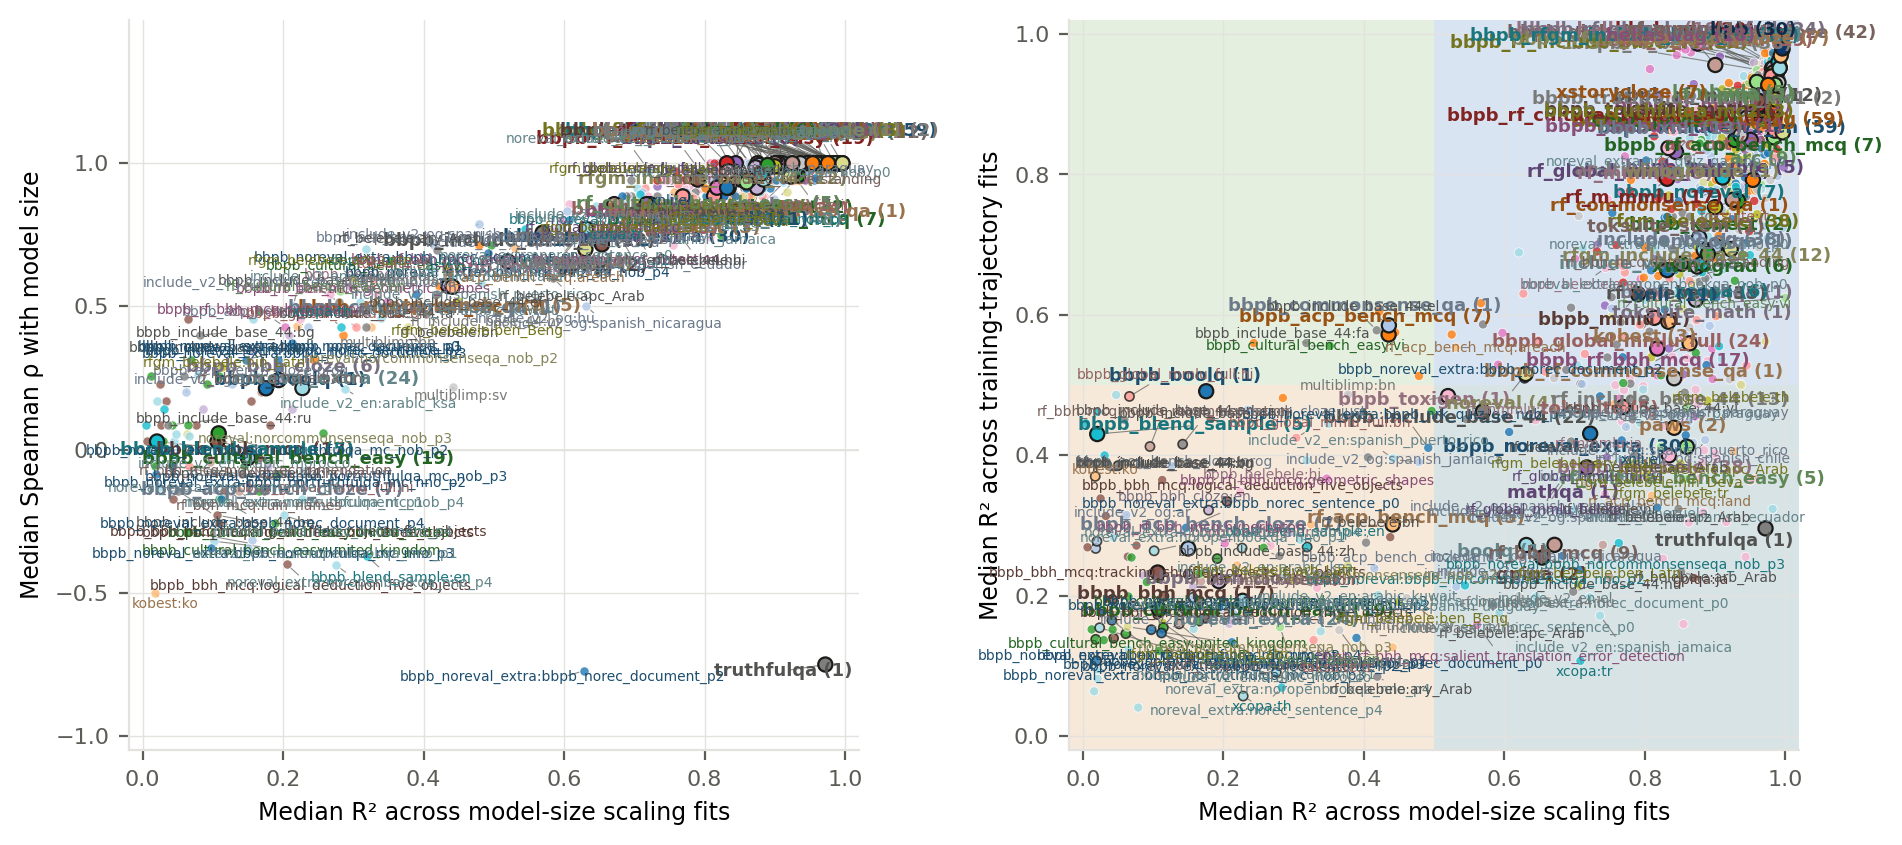
\includegraphics[width=\textwidth,height=0.36\textheight,keepaspectratio]{figures/rq1.png}
% source: src/signal-and-noise/analysis/rq01_scaling_predictability/pretraining/predictivity_seeds/scaling_regimes_outliers_paper.png
\captionof{figure}{\textbf{Accuracy scales log-linearly where it is above chance.} Each point is one benchmark-language task. Left: the median Spearman $\rho$ of the score with model size against the median R$^2$ of the log-linear fits across model size. Right: the median R$^2$ of the fits along training against the same x axis. The shading splits each axis at 0.5. Bold labels name each benchmark family at its median point (its number of tasks in parentheses) and small labels name the outlying tasks.}
\label{fig:app_rq01_scaling_predictability}
\end{minipage}
}]

\begin{figure*}[p]
\centering
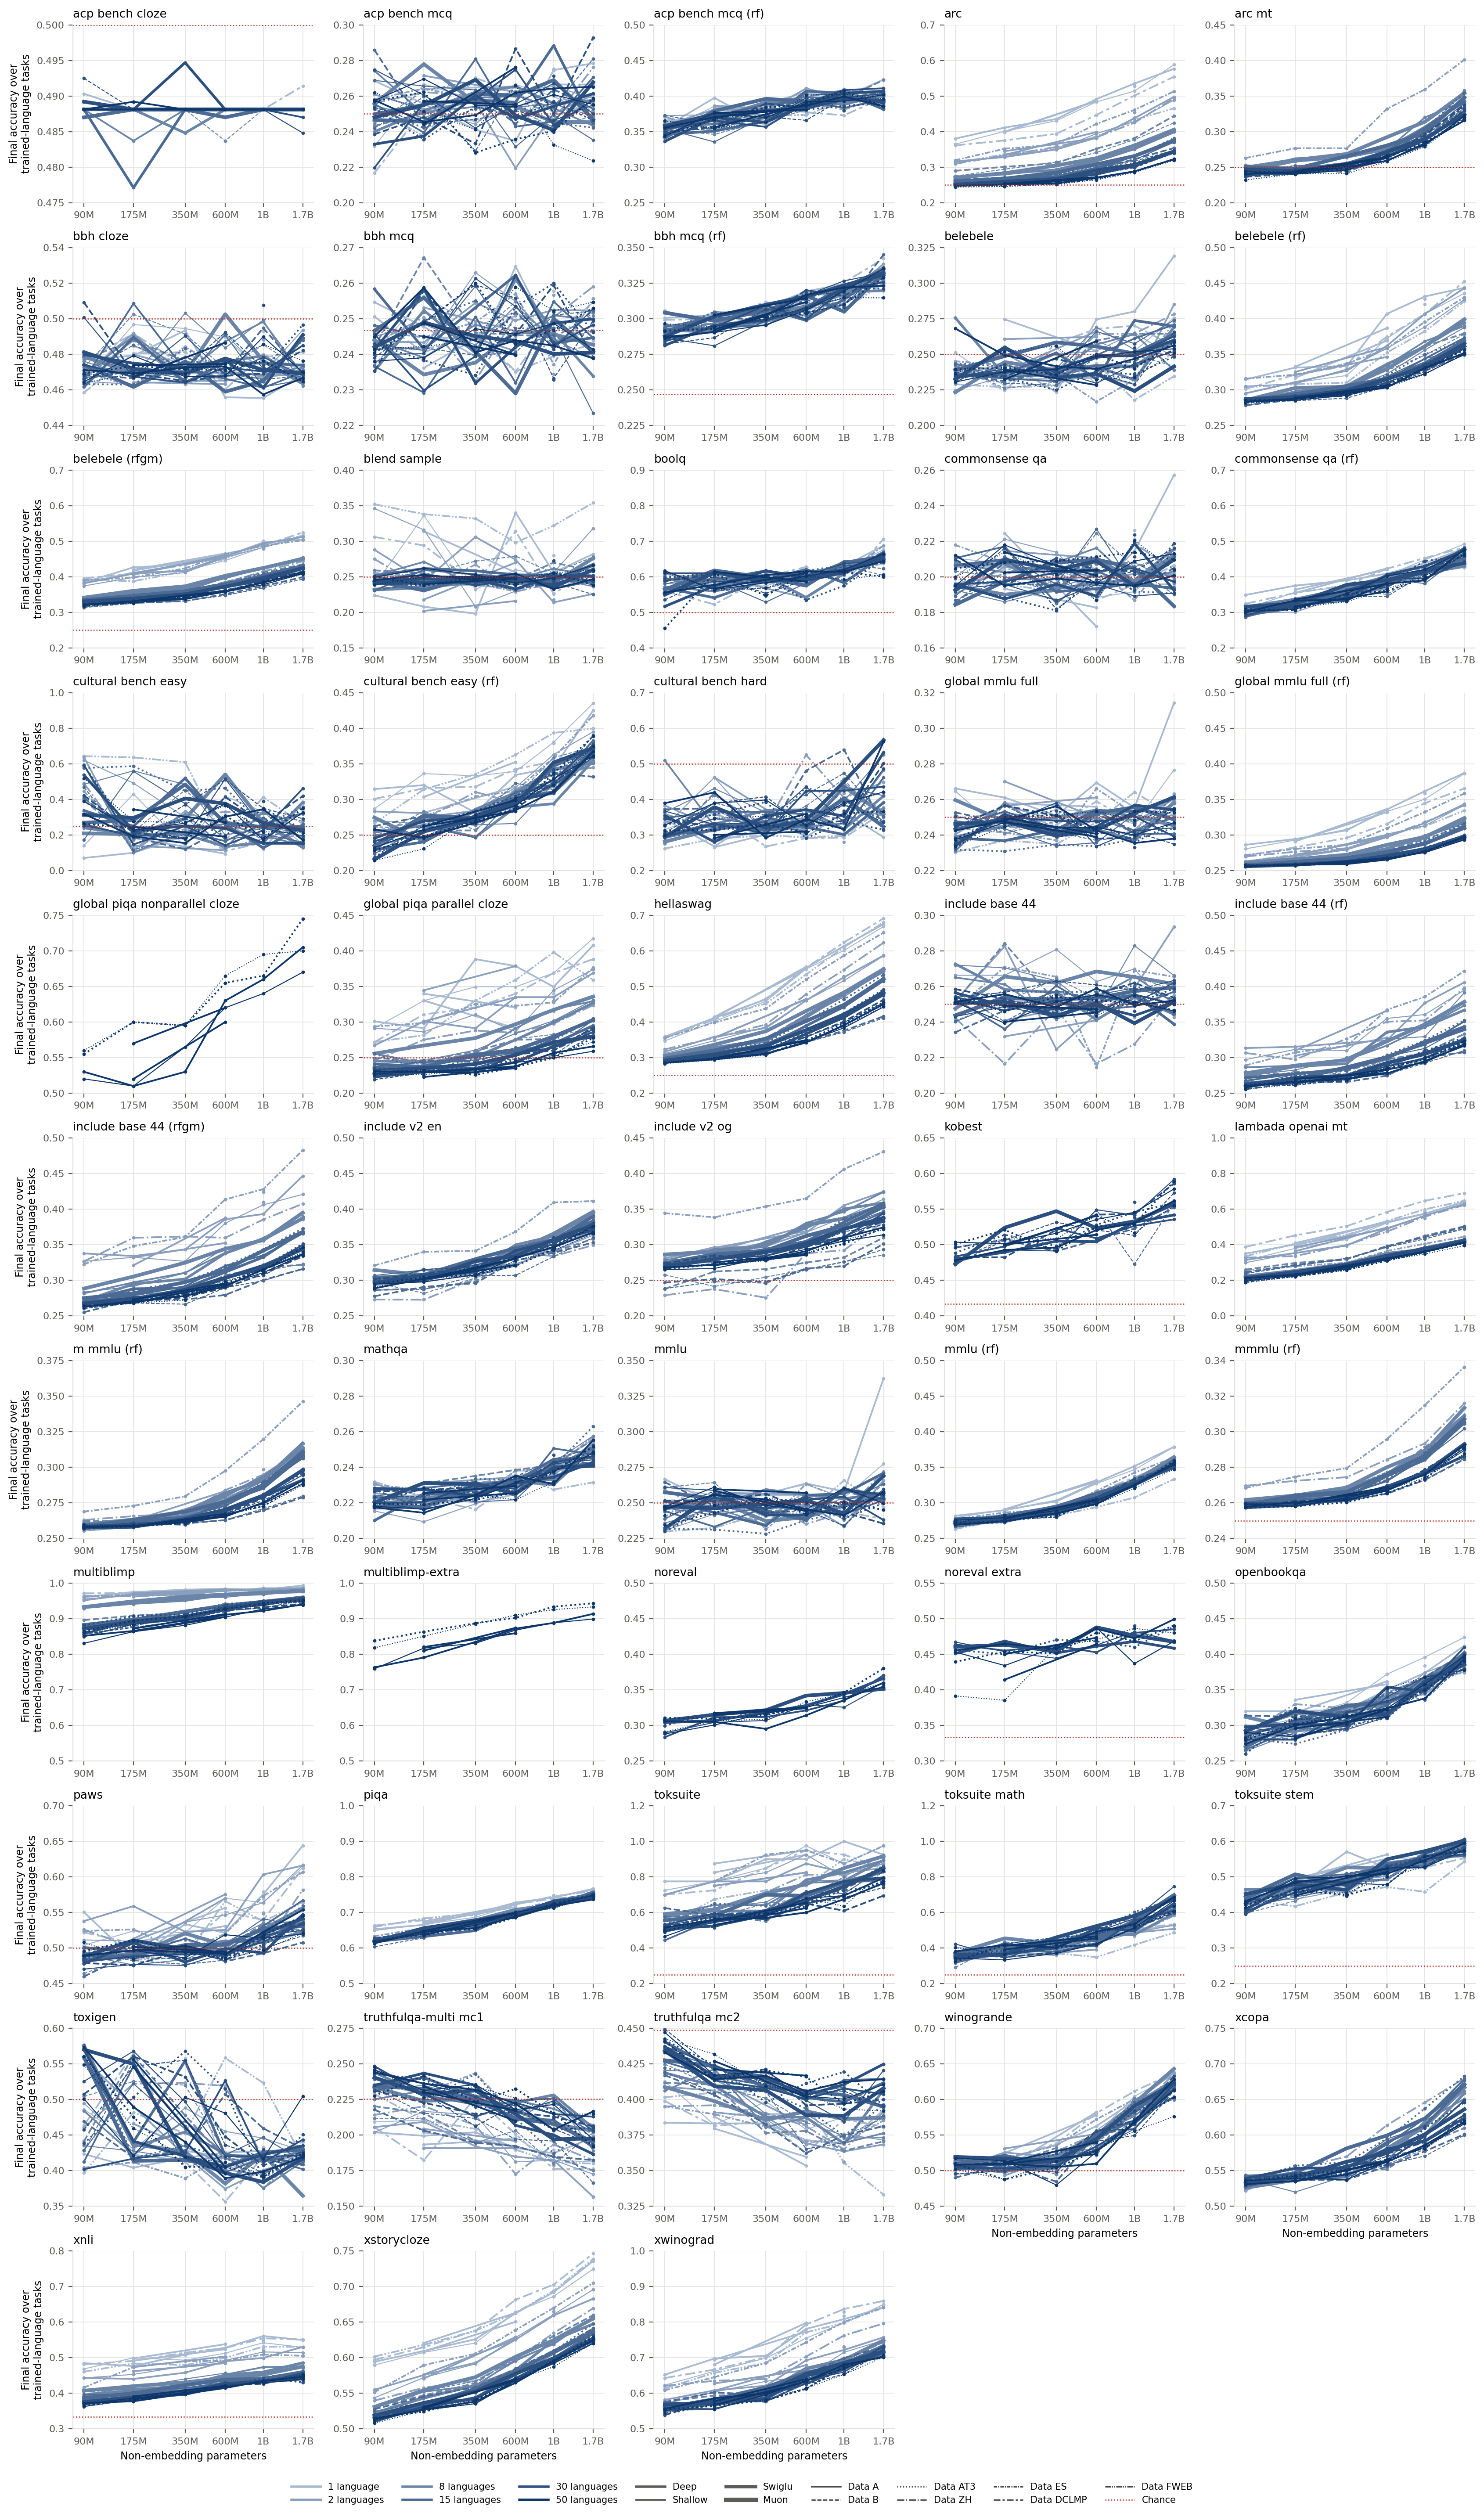
\includegraphics[width=\textwidth,height=0.8\textheight,keepaspectratio]{figures/app_rq00_benchmark_size_curves.png}
% source: src/signal-and-noise/analysis/rq00_gate_and_curves/pretraining/predictivity_seeds/benchmark_size_curves_paper.png
\caption{\textbf{The reformulated twins rise with model size while their letter-format originals stay at chance up to 1.7B.} Benchmark accuracy against model size. For each benchmark family, we plot the final-checkpoint accuracy of every design against non-embedding parameters. This accuracy is the mean over the tasks in the languages the design trains on. There is one line per (number of languages, ladder, data build, seed), over 90M--1.7B. Colour gives the number of trained languages, line width the ladder and line style the data build. The dotted red line is chance. The curves are not gated, so a family at chance stays visible.}
\label{fig:app_size_scaling}
\end{figure*}

\begin{figure*}[p]
\centering
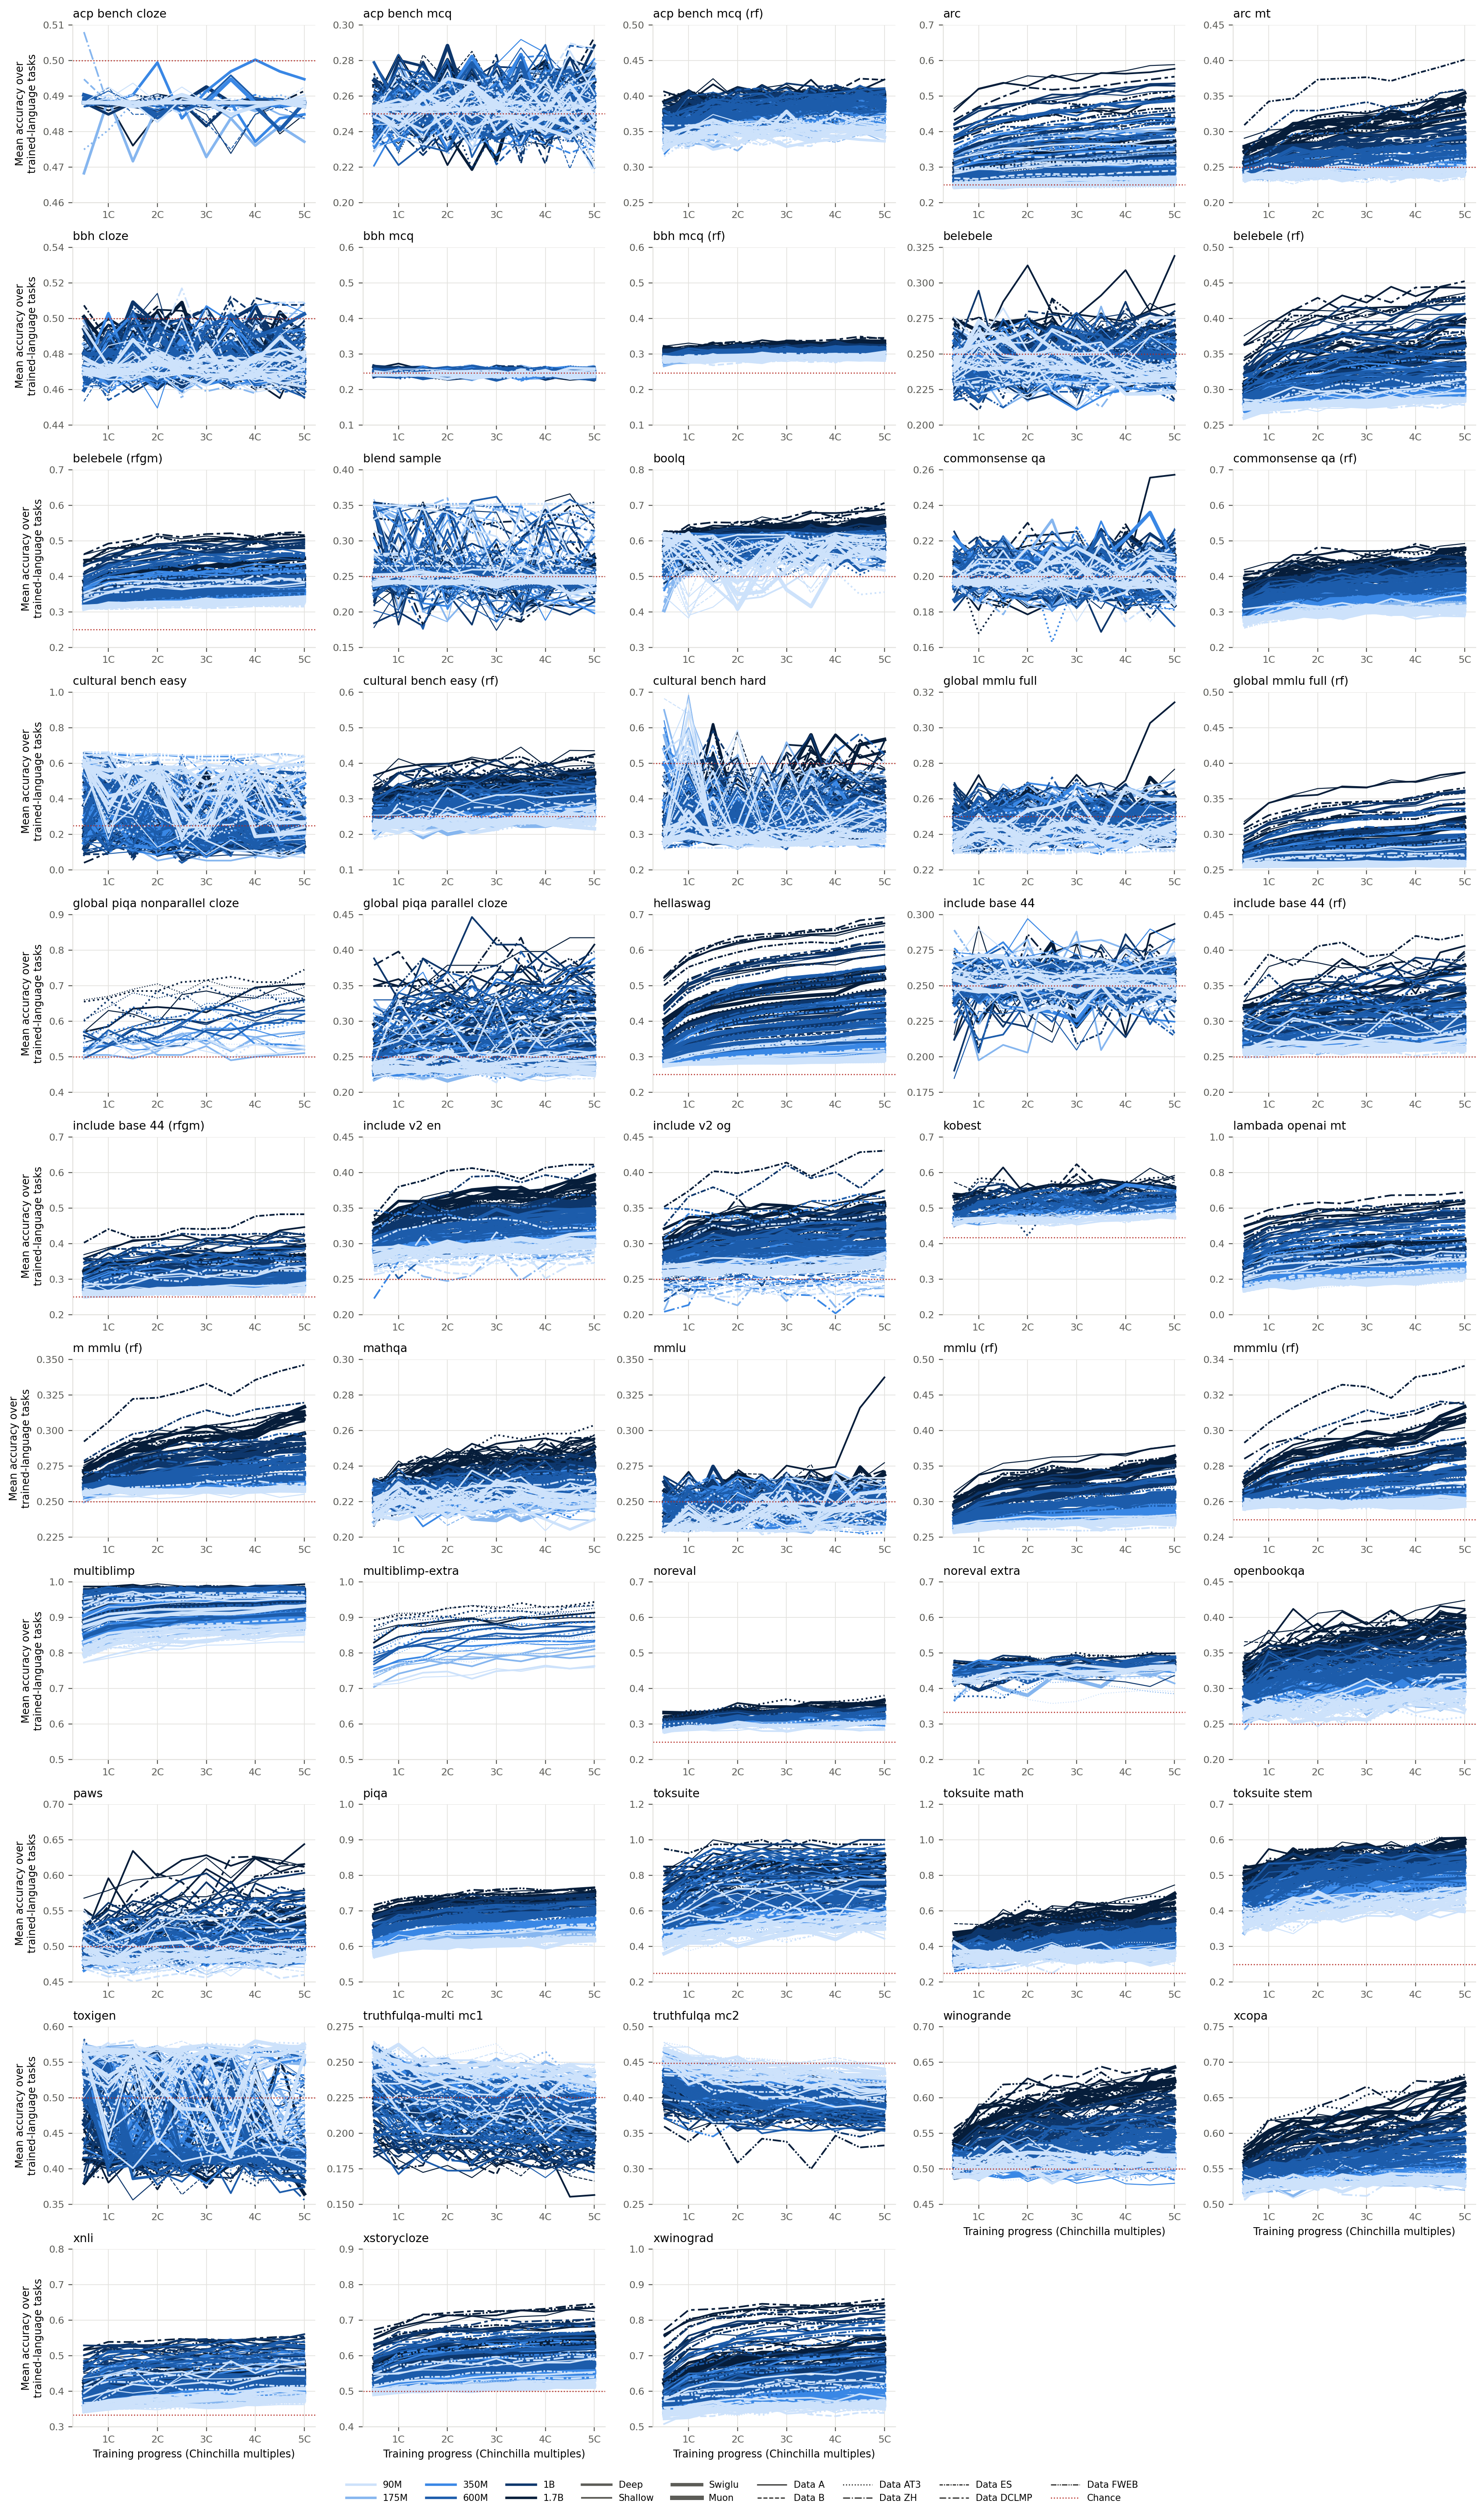
\includegraphics[width=\textwidth,height=0.8\textheight,keepaspectratio]{figures/app_rq00_benchmark_curves.png}
% source: src/signal-and-noise/analysis/rq00_gate_and_curves/pretraining/predictivity_seeds/benchmark_curves_paper.png
\caption{\textbf{Along training, the letter-format originals stay at chance for the whole run while their reformulated twins climb steadily.} Benchmark accuracy along training. For each benchmark family, we plot the accuracy of every run at the ten evaluated tenths of the run. This accuracy is the mean over the tasks in the languages the run trains on. Training progress is given in Chinchilla multiples of the run's token budget. The figure covers every seed and data build, 90M--1.7B. Colour gives the model size, line width the ladder and line style the data build. The dotted red line is chance. The curves are not gated.}
\label{fig:app_training_scaling}
\end{figure*}
